\documentclass[12pt, a4paper]{article}
\usepackage{pdflscape} %Landscape format

\usepackage{graphicx}
\graphicspath{ {./images/} }

\usepackage[ddmmyyyy]{datetime}
\renewcommand{\dateseparator}{.}
\renewcommand{\figurename}{Şekil}
\renewcommand{\refname}{Kaynaça}
\usepackage{url}


\begin{document}

\textbf{KÜTAHYA SAĞLIK BİLİMLERİ ÜNİVERSİTESİ
MÜHENDİSLİK VE DOĞA BÖLÜMLERİ FAKÜLTESİ}\centering \\[20pt]

\begin{figure}[!h]
	\centering
	
\includegraphics{ksbu.png}
	\\[20pt]
\end{figure}

\textbf{YAPAY ZEKA DERSİ}\centering\\[20pt]
		
\textbf{NÖBET ÇİZELGELEME PROBLEMLERİNİN GENETİK ALGORİTMALARLA OPTİMİZASYONU}\centering\\[15pt]
		
\textbf{Mustafa AKER} \\[10pt] 
\textbf{2118121039} \\[10pt]
\textbf{\today}

	
	
	

	\newpage	
		
\begin{flushleft}
   \section{Giriş}	
   Optimizasyon, bir sistemi veya süreci en iyi duruma getirmek için yapılan bir dizi işlem veya stratejidir. Genellikle belirli bir hedefin veya kriterin en iyi şekilde karşılanması için kaynakların en verimli şekilde kullanılmasını içerir \\[5pt]
   Çizelgeleme problemleri; çalışanların en düşük işgücü maliyetleri ile çalışma vardiyalarına	atanmasının belirlenmesini, personel hizmet kalitesi ve çalışma yasalarıyla ilgili 
   kısıtlamaların karşılanmasını konu alan problemlerdir.\\[5pt]
   
   Çizelgeleme problemlerinin uygulama alanlarının başında; hastaneler ,sağlık merkezleri,havalimanları,üniveristeler gibi bir cok kurum gelmektedir. Kurumların her türlü unsuru göz önünde bulundurması ve uygun bir çizelge oluşturabilmesi gerekir.\\[5pt] 
   
   Çizelgelemedeki asıl amaç, daha az kaynakla ve daha az sürede, istenilen kriterlere uyacak biçimde problemin çözümüne    ulaşmaktır. Bu sebeple probleminin en kısa sürede , istenilen hedef ve kriterlere uygun  çözülmesini sağlayacak yollar aranacaktır.
 




	\section{Literatür Araştırması}
	
	
	
	\cite{yamamura1993nurse}
	90'ların sonlarında sezgisel arama yöntemleri hemşire çizelgeleme için de kullanılmaya 
	başlanmıştır. Yamamura ve diğerlerinin (1993) çalışmaları, GA ile yapılan ilk hemşire 
   	çizelgeleme uygulamasıdır.\\[10pt]
	
	\cite{bailey1997using} 
    Bailey ve diğerleri (1997), farklı beceri seviyelerine sahip 
	personelin planlanması sorununa Benzetilmiş Tavlama ve GA uygulamıştır. Sonuçlar, 
	optimal veya optimale yakın çözümler üretilebileceğini göstermektedir.\\[10pt]
	

	
	
	\cite{aickelin2004indirect} 
    Aikelin ve diğerlerinin (2004), ele aldıkları yaklaşım, hemşirelerin permütasyonlarına dayanan dolaylı bir kodlama ile programlar oluşturan sezgisel bir kod çözücü kullanmaktır. Sonuçlar, önerilen algoritmanın yüksek	kaliteli çözümler sunabildiğini ve yakın zamanda yayınlanan bir Tabu Arama yaklaşımından daha hızlı ve daha esnek olduğunu ortaya koymaktadır.\\[10pt]
	
	\cite{duenas2009genetic} 
    Duenas ve diğerleri (2009), hemşirelerin tercihlerini içeren çok amaçlı bir 
	çizelgeyi ele almaktadır. Bu tercihler bulanık kümelerle modellenmiştir ve GA ile birleştirilmiş melez bir çözüm yöntemi kullanılmıştır. Sonuçlar, önerilen yaklaşımın iyi kalitede çözümler ürettiğini ve gerçek hayattaki problemlere uygulanabilir olduğunu göstermektedir.\\[10pt] 
	
	
	
	\cite{balekar2013survey} 
	Balekar ve Mhetre (2013), hemşire çizelgeleme	için GA yaklaşımının kullanıldığı çalışmaları toparlayan bir kaynakça sunmuştur.\\[10pt]
	
	\cite{leksakul2014nurse} 
    Leksakul ve Phetsawat çalışmasında elde edilen sonuçlara göre (2014) GA tarafından bulunan hemşire programı,mevcut programla karşılaştırıldığında aylık personel giderlerinde \% 12 ve hemşire sayısında \\ \% 13 tasarruf  görülmüştür.\\[10pt]
	 
	 
	\cite{kim2018genetic}
	Kim ve diğerleri (2018), popülasyon 
	büyüklüğü ve mutasyon oranı parametrelerini dikkate alarak Memetik Algıritma ve GA 
	kıyaslamışlardır.\\[10pt]
	
	\cite{alfadilla2019optimization} 
    Alfadilla ve diğerleri (2019), acil serviste hemşire çizelgelemesi ile 
	ilgilenmişlerdir. GA hemşirelerin yerine getirilmemiş tercihlerini en aza indirmek için 
	kullanılmaktadır.\\[10pt] 
	
	\cite{inancc2020solving} 
	İnanç ve Şenaras (2020), evde bakımda hemşire çizelgeleme problemi için 
	Genetik Algoritma kullanmışlardır.\\[10pt]
	
	\cite{kuccuk2021hemcsire} 
	Küçük ve Deveci Kocakoç (2020) hemşirelerin en uygun çalışma saatlerini bulmak icin  MATLAB programının GA aracından yararlanılmıştır
	
	\newpage	
	\section{Metodoloji}
	Sezgisel algoritmalar 
	genellikle en iyiye yakın olan çözüm yoluna hızlı ve kolay şekilde ulaştıklarından, çalışmada sezgisel algoritmalardan biri olan Genetik Algoritma (GA) kullanılacaktır. GA, tek çözüm değil birden fazla optimal çözüm elde etmesi, çok sayıda parametre ile çalışma imkanı olması, amaç fonksiyonunu geniş bir açıda araştırması nedeniyle yararlı bir yöntemdir. 
	\\[5pt]
	\subsection{Genetik Algoritma }
	Evrimsel hesaplamanın bir alt dalı olan GA ,1970’li yıllarda Michigan 
	Üniversitesi’nden John Holand tarafından bulunmuş ve öğrencileri ile meslektaşlarının 
	yardımıyla geliştirilmiştir. Bunu 1975 yılında Holland’ın “Adaption in Natural and Artificial Systems” adlı kitabını yayınlaması izlemiştir \cite{holland1992adaptation}(Obitko, 1998). GA konusundaki asıl gelişim,John Holland’ın doktora öğrencisi David E. Goldberg tarafından 1985 yılında hazırlanan “Computer-aided gas pipeline operation using genetic algorithms and rule learning” başlıklı doktora tezi ile sağlanmıştır \cite{goldberg1987genetic}(Goldberg ve Kuo, 1987:128)\\[10pt]
	
	İlk kez Lawrence Davis\cite{kelly1991hybrid} tarafından çizelgeleme problemine uygulanan GA, evrim teorisini 
	esas alarak çalışan sezgisel arama algoritmasıdır. En iyi çözüm veya çözümleri bulmaya 
	çalışırken, karar değişkenlerinin genetik sayı sistemindeki kodları ile ilgilenir. Çözümler, kromozomlara benzer bir dizi olarak kodlanır ve bireyler olarak adlandırılır. Algoritma, rastgele üretilen popülasyon adı verilen çözümle başlar. Daha sonra yeni bir popülasyon üretmek için çözümlere genetik operatörler (seçim, çaprazlama, mutasyon ve değiştirme) uygulanır. İşleme, bir durdurma kriteri karşılanana kadar birkaç nesil boyunca devam edilir . Bu operatörlerin işlemleri sonucunda oluşan yeni bireyler, 
	ebeveynlerin bazı özelliklerini taşıyarak çözüme bir adım daha yaklaşan bireylerdir. Belli bir süre sonra popülasyon içerisindeki bireylerin gitgide birbirlerine benzemesinin önüne 
   	geçmek amacıyla yapılan bu işlemler, çözüm uzayının daralmasına engel olmaktadır. 
	
		\subsubsection{Problemin Tanımlanması}
		İlk adım, çözümleme problemi olan çizelgeleme problemi hakkında net bir anlayış geliştirmektir. Bu problem, belirli kısıtlamalara sahip görevlerin bir zaman çizelgesine yerleştirilmesini gerektirir
		\subsubsection{Kromozom Yapısının Tanımlanması}
		Bir çözümü temsil eden kromozomların yapısını tanımlamak önemlidir. Her kromozom, görevlerin sıralamasını içeren bir dizi olabilir. Görevlerin sırasıyla ne zaman başlayacağına karar veren genlerden oluşur.
		\subsubsection{Popülasyonun Oluşturulması}
		 Başlangıçta, belirli bir popülasyon oluşturulur. Her bir birey (kromozom), rastgele bir şekilde oluşturulur.\\[5pt]
		\subsubsection{Uygunluk Fonksiyonunun Tanımlanması}
		Çözümün ne kadar iyi olduğunu değerlendiren bir uygunluk fonksiyonu belirlenir. Bu fonksiyon, çizelgeleme kuralına uyumu ve çözümün kalitesini ölçmek için kullanılır.\\[5pt]
		\subsubsection{Çaprazlama Operatörünün Uygulanması}
		İyi performans gösteren bireyler arasında çaprazlama operatörü uygulanır. Bu, iki ebeveynin kromozomlarının belirli bir noktadan kesilip birleştirilerek yeni bireylerin oluşturulmasını sağlar.\\[5pt]
		\subsubsection{Mutasyon Operatörünün Uygulanması}
		Popülasyondaki çeşitliliği artırmak için mutasyon operatörü uygulanır. Bu, rastgele seçilen genlerin değerlerinin değiştirilmesini içerir
		\subsubsection{Yeni Nesli Oluşturulması}
		Çaprazlama ve mutasyon işlemlerinin ardından yeni nesil oluşturulur.\\
		\subsubsection{Uygunluk Değerlerine Göre Seçim Yapılması}
		Oluşturulan yeni nesilden uygunluk değerlerine göre en iyiler seçilmesi ve bir sonraki iterasyon için kullanılması.
		
		\subsubsection{Durdurma Kriterlerinin Belirlenmesi}
		Algoritmanın ne zaman duracağını belirlemek için bir durdurma kriteri belirlenir. Bu, belirli bir uygunluk seviyesine ulaşılması veya belirli bir iterasyon sayısına ulaşılması olabilir.
		\subsubsection{Sonuçların Değerlendirilmesi}
		Algoritmanın sonuçlarını değerlendirerek çözümün uygunluğu kontrol edilir.\\[30pt]
	
	
	\section{ Veri Ve Sistem Tasarımı}
    	\subsection{Veri Toplama}
    	Projede veri olarak \cite{evliyacelebieah.saglik.gov.tr} Kütahya Sağlık Bilimleri Üniversitesi Evliya Çelebi Eğitim Ve Araştırma Hastanesinin Dahiliye Bölümünde görev yapan hemşirelerin 2024 Mart ayına ait calışma cizelgesi kullanılacaktır.Söz konusu veriler sorumlu kişiler tarafından alınacaktır	\\[10pt]
	
    	\subsection{Kısıtlamaların Belirlenmesi}
    	Hastane yönetimi amaclarına ,personel isteklerine  ve yasal düzenlemelere göre kısıtlar oluşturulacaktır.\\[10pt]
	    \subsection{Algoritmanın Kullanılamsı}
    	Projede kullanılacak olan Genetik Algoritma yöntemi araştırılacak.Veriler ve Kısıtlamalar kullanılarak Phyton dilinde bir model geliştirilecektir. \\[10pt] 
    	\subsection{Test ve Değerlendirme}
    	Geliştirilen modelin çıktıları test edilip değerlendirilecektir \\[10pt] 
	    \subsection{Hata Ayıklama Ve Raporlama}
	    Değerlendirmeler sonucu hata tesbiti ve düzeltmeler yapılacaktır.Projenin son hali raporlanacaktır	\\[10pt] 
	
	\section{Yapılan Projeden Beklentiler} 
	   Yasal düzenlemelere ve kurumların amaçlarına uygun kısıtların sağlanmasının yanında, personel isteklerini karşılayarak onların memnuniyetlerini arttıracak aynı zamanda hizmet alanların ihtiyaçlarını karşılayacak işgücü planlarını ve çizelgeleri oluşturmaktır
	
	%Kaynakçayı yazdırmak
	\bibliographystyle{ieeetr}
	\bibliography{references.bib} 
	%\printbibliography %Prints bibliography
	\end{flushleft}
	 \newpage
	\begin{landscape}
	\begin{figure}
		\centering
		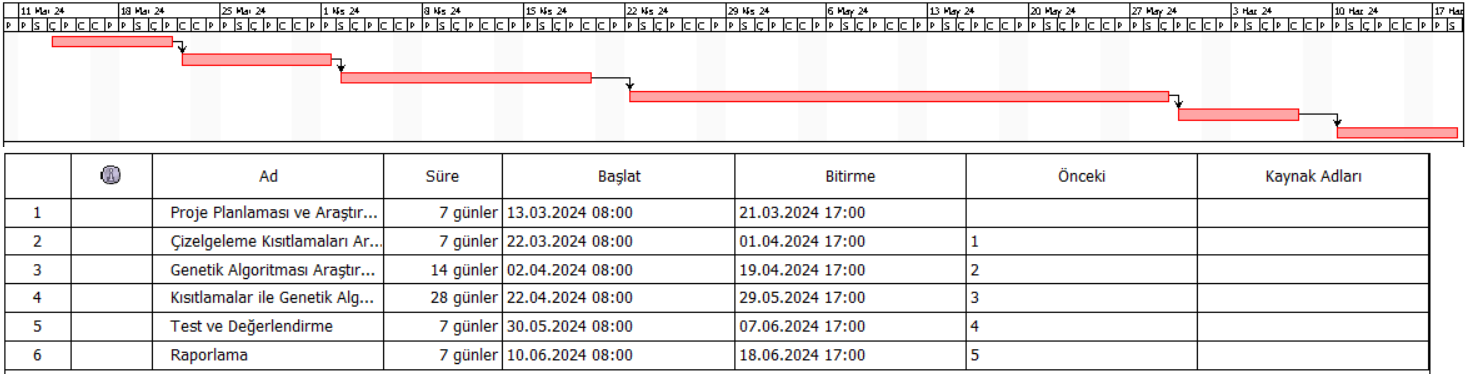
\includegraphics[width=1.5\textwidth]{GantChart.png}
	\end{figure}
    \end{landscape}
	\end{document}